\documentclass[Arkitektur/System_main.tex]{subfiles}
\begin{document}
\subsubsection{Login for bruger}
Når en bruger har lavet en bruger profil skal han herefter logge ind for at kunne udleje sin bil gennem applikationen eller leje en bil fra en udlejer. Til at beskrive denne funktionalitet er der lavet et klassediagram og en statemachine, som kan ses nedenfor. På figur \ref{fig:LoginCD} ses klassediagrammet og på figur \ref{fig:LoginSTM} ses statemachine.

\begin{figure}[H]
    \centering
    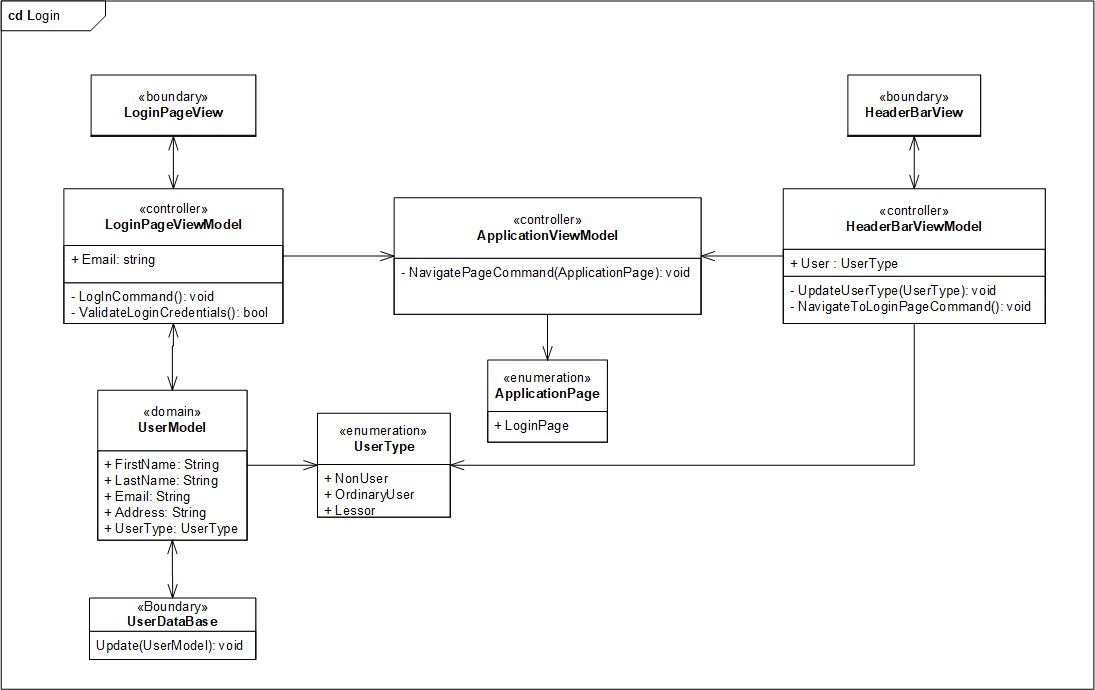
\includegraphics[width=\textwidth]{Arkitektur/Softwarearkitektur/User_Login/graphics/LoginCD.png}
    \caption{Klassediagram for bruger login. }
    \label{fig:LoginCD}
\end{figure}

\begin{figure}[H]
    \centering
    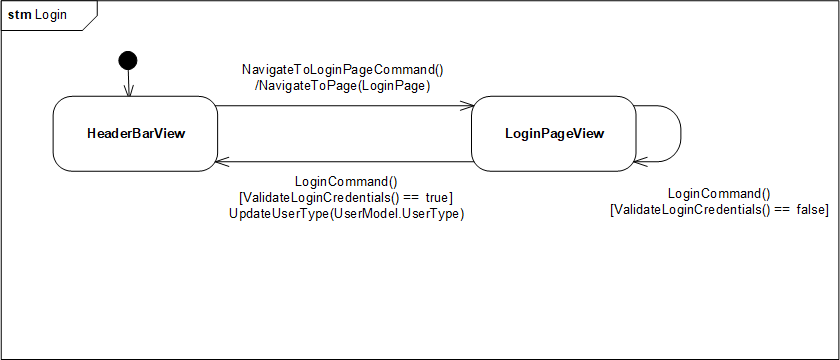
\includegraphics[width=\textwidth]{Arkitektur/Softwarearkitektur/User_Login/graphics/LoginSTM.png}
    \caption{Statemachinediagram for bruger login. }
    \label{fig:LoginSTM}
\end{figure}

\end{document}